\documentclass[12pt,a4paper,oneside,titlepage]{report}
\usepackage{lipsum} %para gerar alguns textos como exemplo
%%%%%%%%%%%%%%%%%%%%%%%%%%%%%%%%%%%%%%%%%%%%%%%%%%%%%%%%%%%%%%%%%%%%%%%%

%Packages(Módulos específicos)

%\usepackage[portuguese]{babel} %para portugues portugal
\usepackage[brazil]{babel} %para portugues brasil
\usepackage[T1]{fontenc} 
\usepackage[utf8]{inputenc}
%\usepackage[latin1]{inputenc}
\usepackage[table,xcdraw]{xcolor}
%\usepackage{setspace} %espaçamento entre linhas
%\renewcommand{\baselinestretch}{1.5} % Espaço entre as linhas
%\usepackage[top=3cm,left=3cm,right=2cm,bottom=2cm]{geometry} %definir margens
%\setlength{\columnsep}{1cm} %para espaçamento de colunas

\usepackage{color,graphicx} %permite a inserção de figuras
\usepackage{lineno} %usamos este pacote para retirar o espaço em branco ao redor das figuras

%%%%%%%%%%%%%%%%%%%%%%%%%%%%%%%%%%%%%%%%%%%%%%%%%%%%%%%%%%%%%%%%%%%%%%%%
%%%%%%%%%%%%%%%%%%%%%%%%%%%%%%%%%%%%%%%%%%%%%%%%%%%%%%%%%%%%%%%%%%%%%%%%

%Abertura

%Introdução do título.
\title{FIGURAS, TABELAS E FÓRMULAS MATEMÁTICAS EM \LaTeX}

%Introdução do autor.
\author{Rosana Massahud}

%Definição da data
\date{\today}

%%%%%%%%%%%%%%%%%%%%%%%%%%%%%%%%%%%%%%%%%%%%%%%%%%%%%%%%%%%%%%%%%%%%%%%%
%%%%%%%%%%%%%%%%%%%%%%%%%%%%%%%%%%%%%%%%%%%%%%%%%%%%%%%%%%%%%%%%%%%%%%%%

\begin{document}

%Gerar o título
\clearpage\maketitle
%\thispagestyle{empty}
%\newpage
%\thispagestyle{empty}
\listoffigures
%\newpage
%\thispagestyle{empty}
\listoftables
%\newpage
%\thispagestyle{empty}
\tableofcontents
%\newpage

%\pagestyle{myheadings} 

% permite ao autor especificar o que ser´a colocado no cabeçalho das paginas. Pode ser de duas maneiras:
% \markboth{pagina par}{pagina impar} %especifica o que sera colocado nas paginas pares e
% impares de acordo com as argumentos do comando.
%\markright{Testando o uso do myheadings} % especifica o que vai no cabe¸calho das paginas pares e impares

%\setcounter{page}{1}
\chapter{Primeiro capítulo}
\section{Primeira seção}

Este é um texto em \textbf{negrito}, \textit{itálico}, \emph{ênfase}, \underline{sublinhado} e em cores.

\lipsum[1-2]
\definecolor{airforceblue}{rgb}{0.36, 0.54, 0.66}
\color{airforceblue}\lipsum[1-2]
\color{red}\lipsum[1-1]
\color{black}


\section{Inserção de figuras}
\begin{flushleft}
\lipsum[1-2]
\end{flushleft}

Na \textbf{Figura} \ref{fig:cachorro} temos um cachorro.


\includegraphics[scale=0.5]{figuras/droopy.jpg}

\begin{figure}[!ht]
\centering 
\includegraphics[scale=0.5]{figuras/droopy.jpg}
%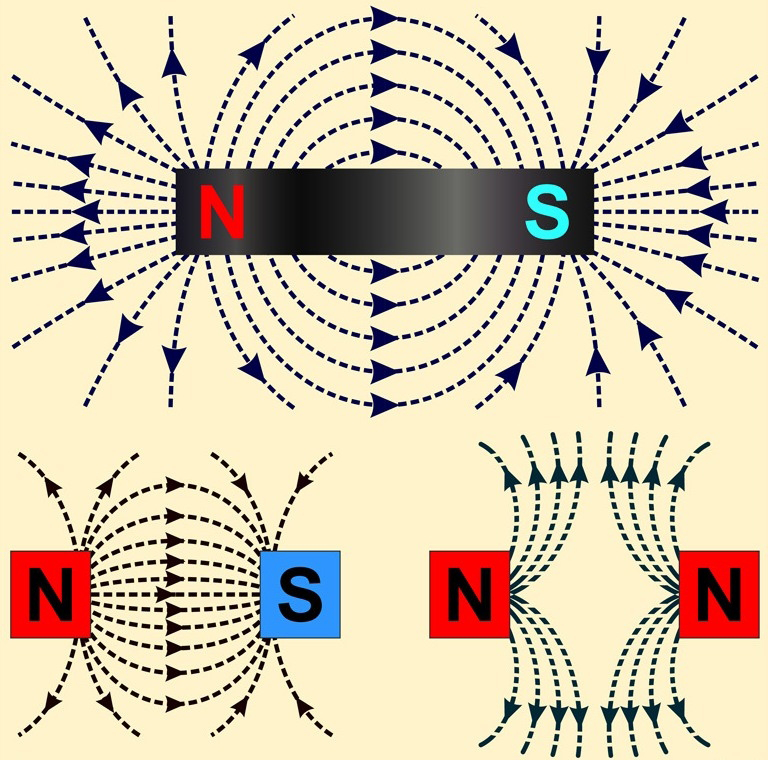
\includegraphics[scale=0.5]{figuras/figura1.eps}
\caption{Título da figura}\label{fig:cachorro}
\end{figure}

Este parágrafo mostra um exemplo de como podemos nos referenciar a uma figura no texto, através de sua \textit{label}. Por exemplo, na \figurename{ \ref{fig:cachorro}} temos um cachorro, que eu esqueci qual o nome dele.

Uma outra figura pode ser vista abaixo (\figurename{ \ref{fig:grafico}}).

\begin{figure}[!ht]
\centering 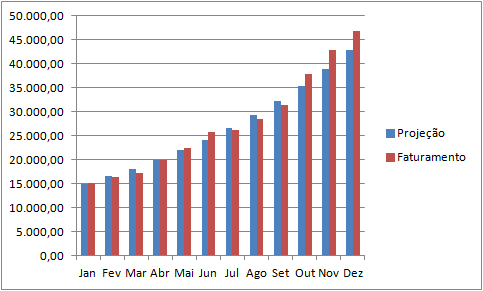
\includegraphics[scale=0.5]{figuras/grafico.jpg}
%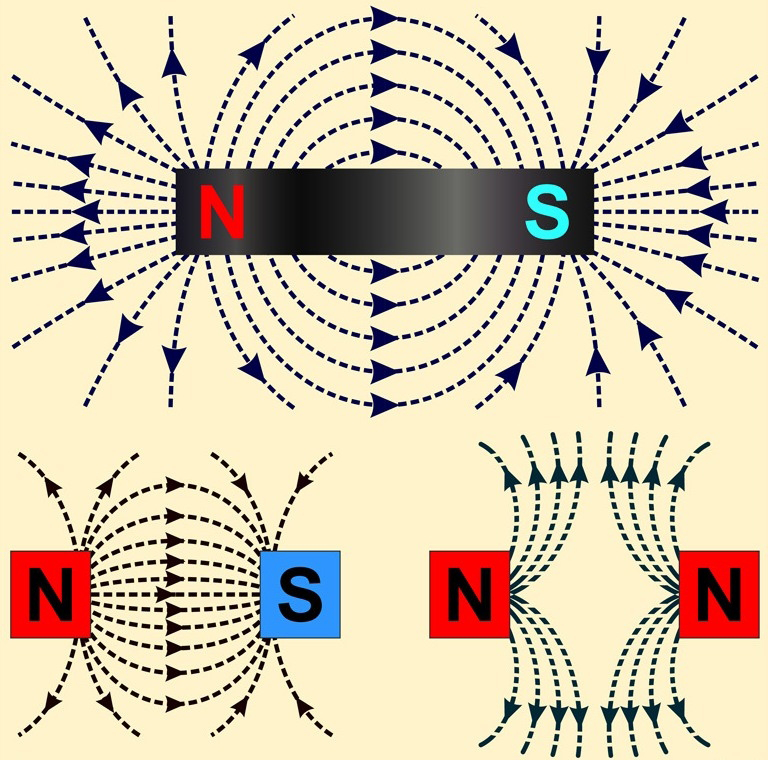
\includegraphics[scale=0.5]{figuras/figura1.eps}
\caption{Exemplo de um gráfico}\label{fig:grafico}
\end{figure}

\lipsum[1-2]

\section{Tabelas}
\lipsum[1-1]

\begin{table}[h!]
\caption{Exemplo de tabela simples}
\begin{center}
\begin{tabular}{|c|c|}
\hline 
algum texto & coluna 2 linha 1 \\ 
\hline 
coluna 1 linha 2 & outro texto \\ 
\hline 
\end{tabular} 
\end{center}
\label{tab:tab1}
\end{table}

\lipsum[1-1]

\begin{table}
\begin{center}
\begin{tabular}{|l|l|l|}
\hline
\multicolumn{1}{|c|}{\textbf{a}} & \multicolumn{1}{c|}{\textbf{b}} & \multicolumn{1}{c|}{\textbf{c}} \\ \hline
1                                & 2                               & 3                               \\ \hline
\end{tabular}
\end{center}
\caption{teste teste}
\end{table}

\section{Fórmulas matemáticas}
Algumas fórmulas matemáticas simples:

Adicione o quadrado de $a$ ao quadrado de $b$ para obter o quadrado de $c$. Então, fica: $c^2 = a^2+b^2$. Ou, usando uma notação mais matemática: 
\begin{displaymath}
c^{2}=a^{2}+b^{2}
\end{displaymath}


\[
a_n = a_1*(n-1)*r
\]
E apenas uma linha a mais.

$\Delta = b^2 - 4\cdot a \cdot c$

O ambiente é delimitado por \$ \$ ou \verb|\begin{math} \end{math}|.

Alguns exemplos de equações:

	$\lim_{n \to \infty} \sum_{k=1}^n \frac{1}{K^2} = \frac{\pi^2}{6}$

	\begin{displaymath}
		\lim_{n \to \infty} \sum_{k=1}^n \frac{1}{K^2} = \frac{\pi^2}{6}
	\end{displaymath}

Um exemplo de como podemos nos referenciar à uma equação no texto\dots

Segundo a Equação \ref{eq:ex1}, blá blá blá \dots

	\begin{equation}
		\lim_{n \to \infty} \sum_{k=1}^n \frac{1}{K^2} = \frac{\pi^2}{6}				
		\label{eq:ex1}		
	\end{equation}

\textbf{Matrizes}

	\begin{displaymath}
	M = \left (
			   \begin{array}{ccc}
				x_{11} & x_{21} & \ldots \\
				x_{21} & x_{22} & \ldots \\
				\vdots & \vdots & \ddots
			   \end{array}
		  \right)
	\end{displaymath}

	\begin{displaymath}
		A = \left[ \begin{array}{ccc}
					-1 & 2  & 3 \\ 
 					3 & 5 & -6\\
 					2 & 1  & -4
				\end{array} \right]
	\end{displaymath}

\begin{displaymath}
det_A = \left| \begin{array}{rcr}
-1 & 2  & 3 \\ 
 3 & 5 & -6\\
 2 & 1  & -4
\end{array} \right|
\end{displaymath}

	Segundo a equação \ref{eq:equacao1}...
	\begin{equation}\label{eq:equacao1}
		a^2=c^2
	\end{equation}


	Segundo a equação \ref{eq:equacao2}...
	\begin{equation}\label{eq:equacao2}
		a^2=c^2+ 45
	\end{equation}


\textbf{Sistemas de equações}
\\
\\
\begin{equation}
\left\{
\begin{array}{l l}
2x+3y+2z=13\\
x-z=1
\end{array}
\right.
\end{equation}
\\

$
\left\{
\begin{array}{lll}
x+3y+4z+12w=0\\
x+y-2w=10\\
-x+12w=11
\end{array}
\right.
$
\\

\begin{equation}
f(n) =
\left\{ 
\begin{array} {ll}
n, \mbox{se }n\mbox{ é par}  \\ 
3n+1, \mbox{se }n\mbox{ é ímpar} 
\end{array} 
\right.
\end{equation}

\textbf{Derivadas e Integrais}

\[ 
\frac{\partial f}{\partial x}(a,b) = \lim_{h \to 0} \frac{f(a+h,b)-
f(a,b)}{h} 
\]

\[ A= \int \! \! \! \int_D \sqrt{x^2-y^2} dx \, dy \]

\[ \oint_C u(x,y) dx + v(x,y)dy \]

\textbf{Vetores}
\\

$ \vec v=2 \vec a + \vec b - 3 \vec c $
\\
\\
$\hat a \ \bar b \ \vec c \ \overrightarrow{a b} \ \overleftarrow{c d} \ \widehat{d e f} \ \overline{g h i} \ \underline{j k l}$


\end{document}